%# -*- coding: utf-8-unix -*-
%%==================================================
%% chapter05.tex
%%==================================================

%\bibliographystyle{sjtu2}%[此处用于每章都生产参考文献]
\chapter{系统架构与开发实现}
\label{chap:design_and_implement}
本系统基于敏捷开发、响应式设计、Flux架构模式等理论指导,在简洁且充分的需求分析的基础之上,使用全栈JS技术和各类高效的开发工具开始了系统设计与开发。三个模块使用的各类理论、技术和工具互有重叠:
\begin{itemize}
  \item 在开发模式方面,都是使用的敏捷开发,频繁部署新版本的同时不断地根据需求和反馈迭代开发。
  \item 在UI设计和页面布局方面,都使用了Flex布局和google的Material design,程序员能够方便地控制页面布局,同时页面也简洁美观富有质感。
  \item 在API设计方面,各有一套RESTful风格的API让APP能够方便地增删改查各类资源,同时WebSocket的使用让APP能够及时地获得数据更新。
  \item 在权限校验方面,在Oauth和JWT的帮助下,用户能够安全、方便地访问我们的系统,将来系统也很容易加上单点认证系统或者接入其他第三方平台。
  \item 在版本控制和代码风格方面,都使用了Git和Git flow来控制版本和发布,使用了JSCS、stylelint、pre-commit和代码审查来保证代码风格的一致。
  \item 在测试方面,都选择了Karma+Mocha+Chai+Sinon的技术栈,加上Solano CI来持续集成和自动部署。
\end{itemize}
\section{版本管理模块}
本模块使用基于比较成熟的MEAN技术栈,即MongoDB+ExpressJS+AngularJS+NodeJS。本模块比较特殊的一点在于使用了代码生成器,本文作者也是这个项目的主要代码贡献者之一。另外本模块在页面布局方面额外使用了响应式设计来使得页面能够适应所有大于平板的屏幕宽度,使用了gulp作为构建工具,使用jshint来检查语法,前后端分别使用了Atom和Webstorm来编辑源代码。

下面将主要以用户和传感器两种资源为例,按照资源从后向前传递、从整体到细节展示的顺序,从API、API路由、客户端模型定义和响应式设计几个方面介绍本模块的详细设计与开发,另外还特别介绍了本模块使用的代码生成器,最后从Git代码提交记录的角度介绍了本模块和代码生成器的关系。
\subsection{API}
本模块使用RESTful风格的API,包含新建、删除、修改、列表查询和单一查询五种API,围绕Mongoose的数据模型来进行增删改查等业务,同时使用WebSocket在保存和删除的同时发送消息给前端,让前端及时获悉改动。如图4-1所示,这是传感器API完整的目录结构,其中包含controller(业务逻辑控制器)、model(Mongoose数据模型)、params(查询参数)和socket(WebSocket事件注册)以及两个测试文件。
\begin{figure}[H]
 \centering
 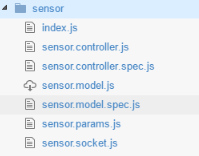
\includegraphics[width=0.4\textwidth]{sensor_api_files.png}
 \bicaption[fig:sensor_api_files]{传感器API目录结构}{传感器API目录结构}{Fig}{Directory of Sensor's API}
\end{figure}
这里的业务逻辑控制器里面其实没有真正的增删改查逻辑,因为增删改查等操作是每个资源的API都应该有的,所以它们被泛化到了控制器的基类CrudController中。如代码4.1所示,CrudController是一个构造函数,接收一个模型(model)作为参数,所以不同的业务逻辑控制器可以传入各自的model就可以使用基类的增删改查函数来注册API了。
\begin{lstlisting}[language={JavaScript}, caption={传感器API定义}]
/* in crud.controller.js */
function CrudController(model) {
  // set the model instance to work on
  this.model = model;
}
/* in sensor.controller.js */
function SensorController(router) {
  // call super constructor
  CrudController.call(this, Sensor,  router);
}
/* in sensor/index.js */
// register sensor routes
router.route('/')
  .get(controller.index)
  .post(controller.create);

router.route('/' + controller.paramString)
  .get(controller.show)
  .delete(controller.destroy)
  .put(controller.update)
  .patch(controller.update);
\end{lstlisting}

如代码4.2所示,本模块在socket文件中给传感器模型的保存和删除操作添加了钩子(hook),一旦保存或删除则用WebSocket发送'sensor:save'或'sensor:remove'的消息并附上保存完或删除前的对象,用以通知前端。
\begin{lstlisting}[language={JavaScript}, caption={Sensor的Mongoose模型}]
/* in sensor.socket.js */
function registerSensorSockets(socket) {
  Sensor.schema.post('save', function (doc) {
    onSave(socket, doc);
  });

  Sensor.schema.post('remove', function (doc) {
    onRemove(socket, doc);
  });
}

function onSave(socket, doc, cb) {
  socket.emit('sensor:save', doc);
}

function onRemove(socket, doc, cb) {
  socket.emit('sensor:remove', doc);
}
\end{lstlisting}

如代码4.3所示,传感器的数据模型通过一个可嵌套的对象来定义。
\begin{lstlisting}[language={JavaScript}, caption={传感器的Mongoose数据模型}]
var SensorDefinition = {
  name: {type: String, required: true},
  hardwareVersion: {type: ObjectId, ref: 'HardwareVersion'},
  firmwareVersion: {type: ObjectId, ref: 'FirmwareVersion'},
  componentBatches: {
    body: {type: ObjectId, ref: 'ComponentBatch'},
    pcb: {type: ObjectId, ref: 'ComponentBatch'},
    photodiode: {type: ObjectId, ref: 'ComponentBatch'},
    laser: {type: ObjectId, ref: 'ComponentBatch'},
    fan: {type: ObjectId, ref: 'ComponentBatch'},
  },
  threshold: {type: Number, required: true},
  noiseLevel: {type: Number, required: true},
  calibrations: {
    mass: Number,
    number: Number
  },
  applicationType: String,
  info: String,
  active: Boolean
};
\end{lstlisting}
\subsection{API路由}
在AngularJS中一个页面由四份代码渲染而成,分别是HTML代码、样式代码、控制器代码和路由器(router)代码。在本模块中把这四份代码分别写在一个文件中,合起来的目录结构叫做一个路由(route);把一套创建、列表、详细和编辑的页面叫做API路由(apiroute),因为它是一套与增删改查API相对应的路由的集合。一个API路由中除了增删改查的基本路由,还有两个抽象路由list和sensor,因为它们的控制器里面几乎没有业务逻辑,HTML代码也不包含任何实际有意义的内容,只是在路由器层面组织起这个结构,特殊的是在这里list路由作为一个插入点对传感器的WebSocket进行了监听,在列表中及时地更新被创建、修改或删除的内容。一个API路由的额外包含一个资源服务(resource service),提供与API交互的所有增删改查函数。

如图4-2所示,这是传感器API路由完整的目录结构,其中sensor.html、sensor.scss、sensor.contoller.js和sensor.js文件分别对应上述四份代码,main、create、detail、edit和items都分别是一个完整的路由,sensor.service.js就是用来定义传感器的资源服务的文件。在这里main路由是create路由和list路由的入口,不作过多介绍。
\begin{figure}[H]
 \centering
 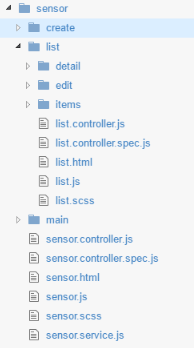
\includegraphics[width=0.4\textwidth]{sensor_files.png}
 \bicaption[fig:sensor_files]{传感器API路由目录结构}{传感器API路由目录结构}{Fig}{Directory of Sensor's apiroute}
\end{figure}

这里以用户页面为例,展示API路由的全貌,如图4-3所示,这套设计让create页面以一个弹窗(modal)的形式浮在list上方;如图4-4和4-5所示,detail页面和edit页面从list右方弹出;如图4-6所示,一旦有数据更新,会有toastr\footnote{一个专门做窗口提示的JavaScript库}窗口提示。
\begin{figure}[H]
 \centering
 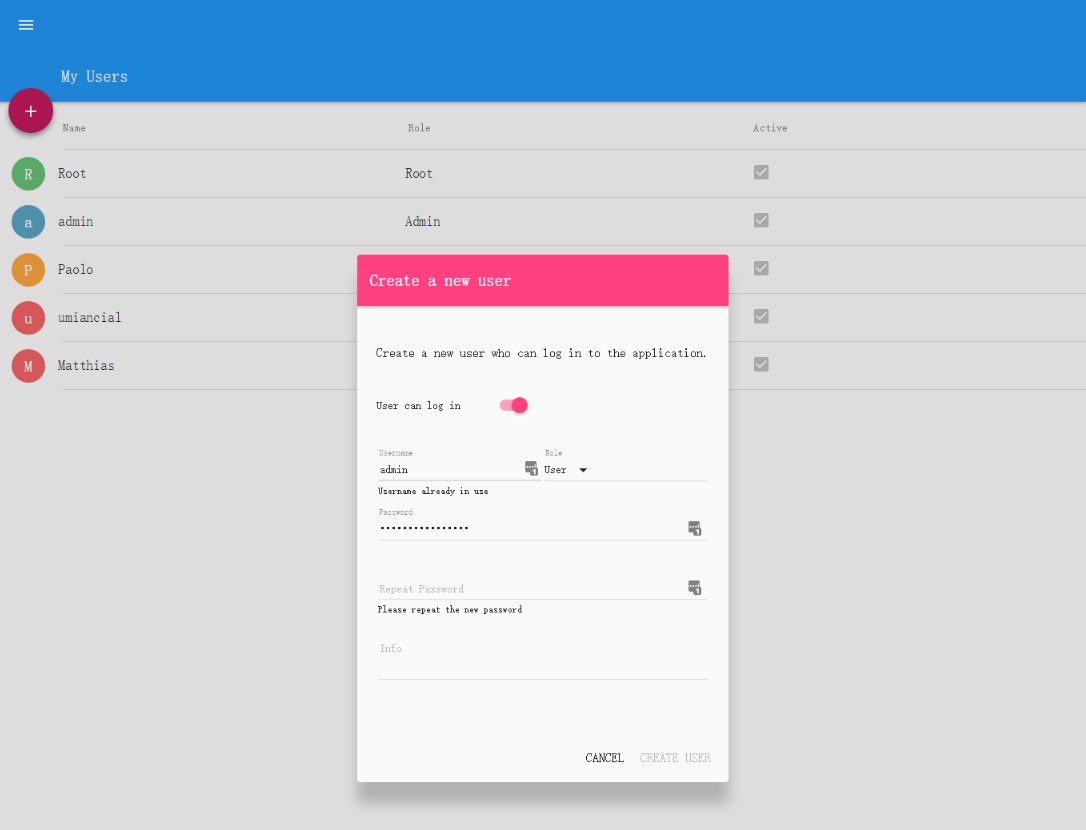
\includegraphics[width=\textwidth]{user_create.png}
 \bicaption[fig:user_create]{用户创建页面}{用户创建页面}{Fig}{Create page of User}
\end{figure}
\begin{figure}[H]
 \centering
 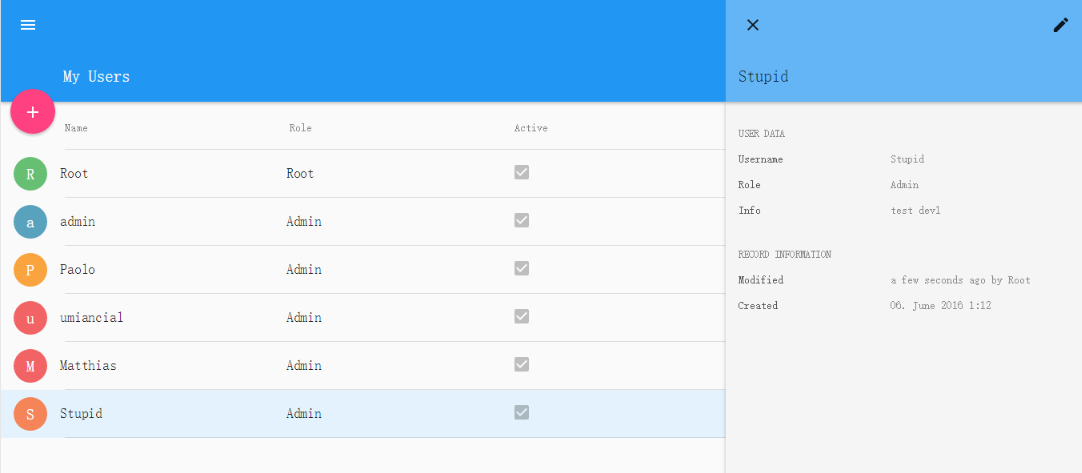
\includegraphics[width=\textwidth]{user_detail.png}
 \bicaption[fig:user_detail]{用户单个查看页面}{用户单个查看页面}{Fig}{Detail page of User}
\end{figure}
\begin{figure}[H]
 \centering
 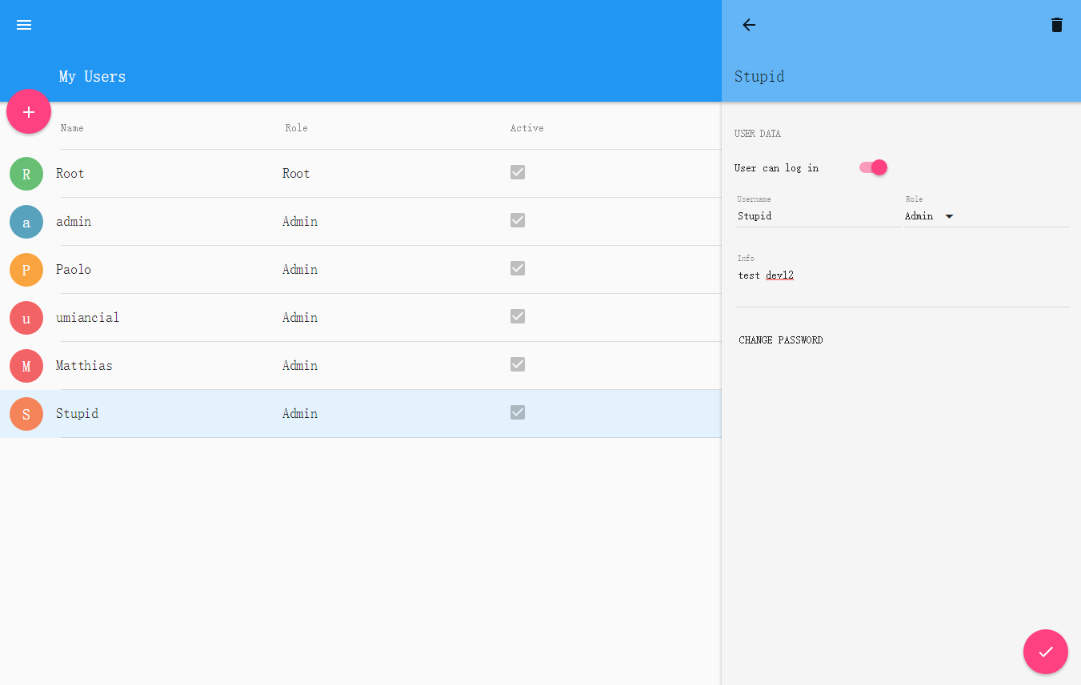
\includegraphics[width=\textwidth]{user_edit.png}
 \bicaption[fig:user_edit]{用户修改页面}{用户修改页面}{Fig}{Edit page of User}
\end{figure}
\begin{figure}[H]
 \centering
 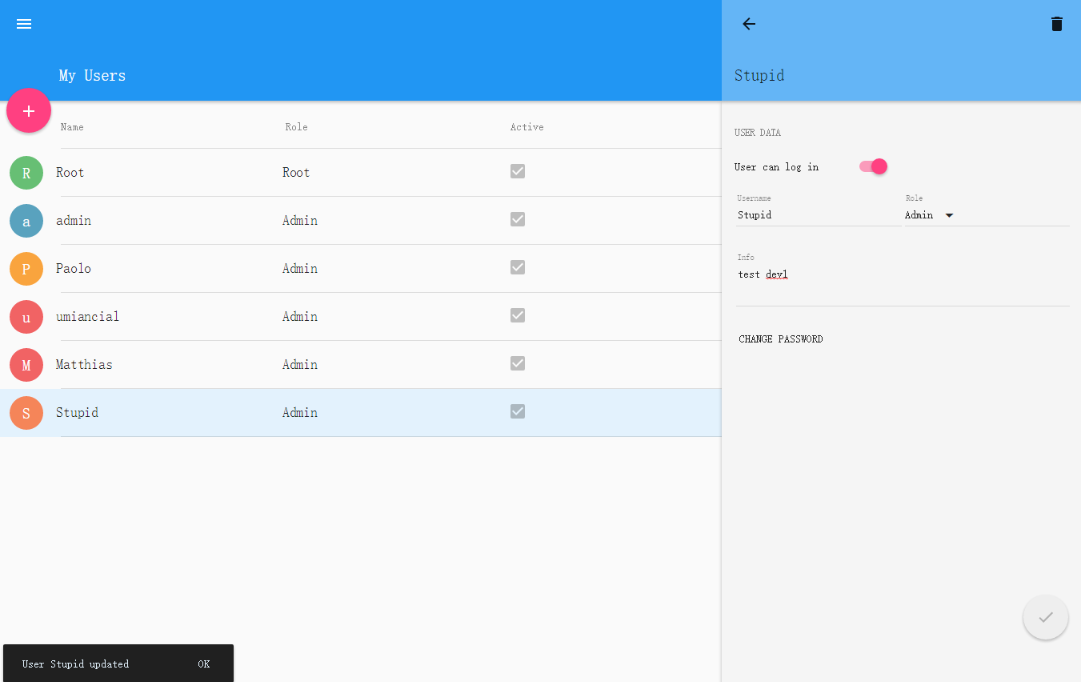
\includegraphics[width=\textwidth]{user_toastr.png}
 \bicaption[fig:user_toastr]{用户提示改动页面}{用户提示改动页面}{Fig}{Toastr box of User}
\end{figure}

\subsection{客户端模型定义}
受Mongoose的基于描述的模型(schema-based model)启发,本模块独创性地自定义了一种客户端模型定义(Client Model Definition),并开发了模型定义服务(ModelDefinitions)和与之配套使用的(当然也可以不使用)两种可重用组件(Angular中的directive)模型输入群组(ModelInputGroup)与模型视图群组(ModelViewGroup)来生成表单、列表和详情页面。

\subsubsection{模型定义服务}
模型定义服务是一个Angular服务(factory),名叫ModelDefinitions。它是一个JavaScript对象函数\footnote{JavaScript中函数也是对象,可以像对象一样拥有属性},作为函数它能够把嵌套的、带有各种简写和别称的模型定义转化为一组扁平化的属性定义(flatten PropDefinitions),如下文中代码4.4里嵌套的calibrations.mass字段会变成一个名叫'calibrations.mass'的属性定义,一个资源的模型定义最终表现形式就是属性定义数组。为方便使用扁平化的名字对模型进行操作,作为对象的模型定义服务还提供有深度扩展(deepExtend)、深度读写(deepGet和deepSet)、深度显示(deepDisplay)等辅助函数,分别是它的属性extend、get、set和display。

对于模型定义的设计,首先模仿了Mongoose模型的类型(type)、必要(required)、引用(ref)三种选项,其中引用在前端定义中是一种资源,所以叫resource。type也有比较大的差异,主要是Mongoose中的基础类型对应地变成了前端input输入框中允许的类型以及特殊的选择类型,
\begin{description}
  \item[input支持的类型] 如text(String)、url(String)、number(Number)、date(Date)、password(String),括号中为对应的Mongoose字段类型;
  \item[select] 因为JavaScript数组是弱类型的,所以select可以对应Mongoose字段的任意类型,具体类型由选项数组中的值的类型来定;
  \item[select/resource] 对应Mongoose中的ObjectId类型,和ref一样另有resource来指定资源。
\end{description}

客户端模型的每个字段除了有与Mongoose类似的类型、必要和资源三个选项外,还有一些用于定义表单输入和页面视图的选项:
\begin{description}
  \item[desc] 字符串,用于显示在输入群组和视图群组中对字段的描述,如果不填,默认为字段名的首字母大写;
  \item[displayKey] 字符串,用于显示在输入群组和视图群组中字段的值,如果字段值为对象,只显示对象中的这个指定字段;
  \item[format] 对象或正则表达式,用于输入群组中的正则格式校验,可以包含正则表达式(value)和出错信息(error)两个选项,也可使用默认出错信息直接缩写为正则表达式;
  \item[remoteUnique] 字符串,字段唯一,值为指定的资源名称,会自动检查此字段有无其他记录含有相同值;
  \item[repeatInput] 字符串,强制重复输入,值为需要重复的字段名,一般与type=password配合使用,用于重复输入密码;
  \item[validators] 对象,用于输入群组中的各类校验,上述required、format、remoteUnique和repeatInput都属于validators中配置项的简写或别号(alias),对应required、pattern、remote-unique和repeat-input;
  \item[displayPriority] 字符串,用于响应式布局的视图群组中决定是否显示字段,具体细节在下面的\textbf{响应式设计}中介绍;
\end{description}

当type为select时,表单中这个字段对应的输入组件不再是普通的输入框(input box)而是下拉列表(dropdown list),上述都是一些通用的选项,还有一些只在下拉列表中起作用的选项:
\begin{description}
  \item[options] 数组,显示在下拉列表中的选项,与displayKey和valueKey配合使用可以做到显示和实际选择的值不同;
  \item[valueKey] 字符串,实际值字段,如果选项是对象,选项在下拉列表中被选中时字段实际被赋予的值;
  \item[getOptions] 函数,异步获取选项,只在下拉列表(dropdown list)被点开时才异步地获取选项;
  \item[resource] 服务对象(service),当资源被指定时,会自动生成getOptions选项,并使用服务对象异步调用查询函数来获取选项数组;
  \item[params] 对象,在使用resource自动生成getOptions选项时,传入查询函数的参数,用于类条件查询;
\end{description}

比如对应上文传感器(Sensor)的Mongoose数据模型,由客户端模型定义的模型如代码4.4所示:
\begin{lstlisting}[language={JavaScript}, caption={Sensor的客户端模型}]
function SensorDefinition (ModelDefinitions, HardwareVersion, FirmwareVersion, ComponentBatch, ComponentTypes) {
    return ModelDefinitions({
      name: {type: 'text', required: true, remoteUnique: 'Sensor', desc: 'ID'},
      hardwareVersion: {
        type: 'select/resource',
        resource: HardwareVersion,
        desc: 'Hardware Version'
      },
      firmwareVersion: {
        type: 'select/resource',
        resource: FirmwareVersion,
        desc: 'Firmware Version'
      },
      componentBatches: {
        body: {
          type: 'select/resource',
          resource: ComponentBatch,
          params: {
            type: ComponentTypes.BODY
          },
          desc: 'Body Batch',
          displayPriority: 'low'
        },
        pcb: {
          type: 'select/resource',
          resource: ComponentBatch,
          params: {
            type: ComponentTypes.PCB
          },
          desc: 'Pcb Batch',
          displayPriority: 'low'
        },
        photodiode: {
          type: 'select/resource',
          resource: ComponentBatch,
          params: {
            type: ComponentTypes.PHOTODIODE
          },
          desc: 'PD Batch',
          displayPriority: 'low'
        },
        laser: {
          type: 'select/resource',
          resource: ComponentBatch,
          params: {
            type: ComponentTypes.LASER
          },
          desc: 'Laser Batch',
          displayPriority: 'low'
        },
        fan: {
          type: 'select/resource',
          resource: ComponentBatch,
          params: {
            type: ComponentTypes.FAN
          },
          desc: 'Fan Batch',
          displayPriority: 'low'
        }
      },
      threshold: {type: 'number', required: true},
      noiseLevel: {
        type: 'number',
        required: true,
        desc: 'Noise Level'
      },
      calibrations: {
        mass: {type: 'number', desc: 'Mass Calibration'},
        number: {type: 'number', desc: 'Number Calibration'}
      }
    });
  }
\end{lstlisting}

\subsubsection{模型输入群组}
模型输入群组(ModelInputGroup)是一个本模块开发的Angular可重用组件(directive),它包含一个模型输入组件(ModelInput),它接收一个Angular模型(ng-model,在组件内部命名为嵌套模型,nestedModel)、一组域定义(fieldDefinitions,因为在表单中所以命名为域定义而不是属性定义)和一个表单对象(form)。模型输入群组会把域定义数组中的每个域定义再传递给模型输入组件。因为域定义是扁平化的,直接按照域定义很难直接管理实际需要的嵌套模型,所以模型输入群组内部额外维护了一个的扁平模型,用户在模型输入组件中输入时直接更新的是扁平模型,然后使用模型定义服务的深度赋值函数对嵌套模型进行修改。如代码4.5所示,只需要插入这样一段调用组件的HTML代码,就可以在传感器资源的创建(create)页面渲染出如图4-7所示的一组输入组件,在修改(edit)页面上也类似。
\begin{lstlisting}[language={HTML5}, caption={传感器创建页面中的模型输入群组代码}]
<model-input-group ng-model="create.sensor"
                   form="createForm"
                   field-definitions="create.sensorDefinition">
</model-input-group>
\end{lstlisting}
\begin{figure}[H]
 \centering
 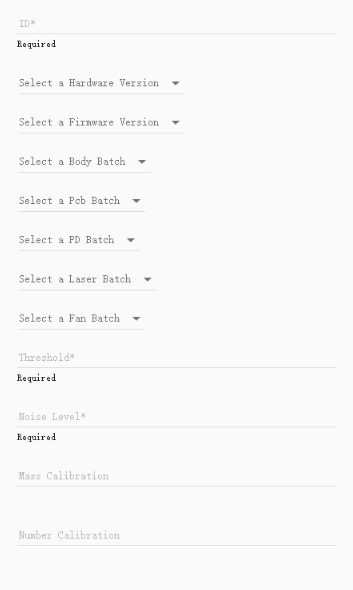
\includegraphics[width=0.6\textwidth]{sensor_create.png}
 \bicaption[fig:sensor_create]{传感器创建页面表单}{传感器创建页面表单}{Fig}{Form in create page of Sensor}
\end{figure}
\subsubsection{模型视图群组}
模型视图群组(ModelViewGroup)也是一个本模块开发的Angular可重用组件,它接收一个模型对象(model,这里不需要修改所以不需要用ng-model)、一组属性定义和一个类型。还有可选项狭窄模式(narrow-mode),用于响应式布局。类型可以分为:
\begin{enumerate}
  \item items-header(列表头部,只横向列出每个属性定义的描述,此类型不需要传入模型对象)
  \item items-content(列表内容,使用模型定义服务的深度显示函数横向列出模型对象每个属性定义的数值)
  \item detail(详细内容,竖向列出属性定义的描述和对应的数值)
\end{enumerate}
如代码4.6所示,只需要插入这样几段调用组件的HTML代码,并且当前app打开了细节页面时(app.inDetailState为true),就可以在传感器资源的列表(list)和细节(detail)页面渲染出如图4-8所示的一组视图组件。
\begin{lstlisting}[language={HTML5}, caption={传感器列表页面中的模型输入群组代码}]
<!-- in items.html -->
<model-view-group definitions="index.sensorDefinition"
                  type="items-header"
                  narrow-mode="app.inDetailState">
</model-view-group>
...
<model-view-group model="sensor"
                  definitions="index.sensorDefinition"
                  type="items-content"
                  narrow-mode="app.inDetailState">
</model-view-group>
<!-- in detail.html -->
<model-view-group model="detail.sensor"
                  definitions="index.sensorDefinition"
                  type="detail">
</model-view-group>
\end{lstlisting}
\begin{figure}[!htp]
 \centering
 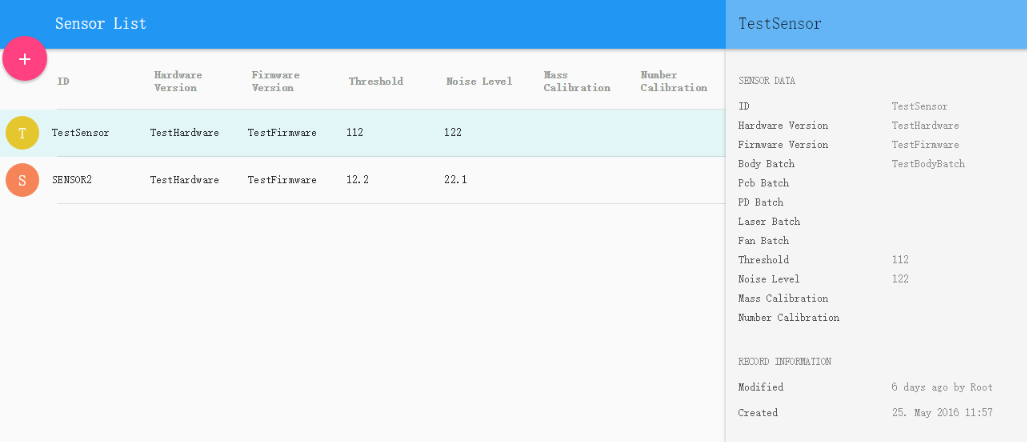
\includegraphics[width=\textwidth]{sensor_detail.png}
 \bicaption[fig:sensor_detail]{传感器细节页面}{传感器细节页面}{Fig}{Detail page of Sensor}
\end{figure}
\subsection{响应式设计}
从上文所展示的列表页面来看,如果一个模型的字段数量过多,或者字段描述过长,不可避免地会在列表的一行内显示不下,由于是flex布局,每个元素根据自己的内容长度都有自己的最小宽度,同时整个页面也有一个最小宽度,因此会出现两种不美观且给用户带来混淆和不便的布局现象,如图4-9,因为某些字段的值过长,整体上列表头和内容不对齐了,如图4-10,编辑页面打开时,因为左边列表页面由最小宽度,所以被挤到屏幕外面去了,要通过横向滚动条才能看到全部的编辑页面。
\begin{figure}[!htp]
 \centering
 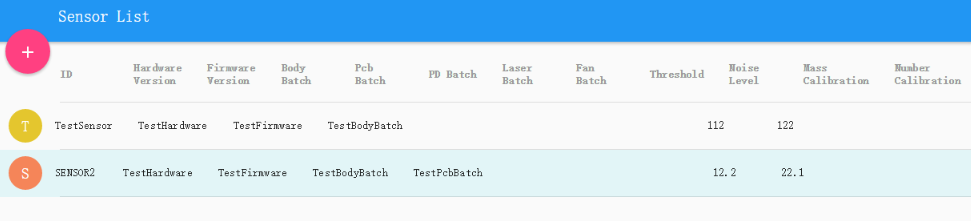
\includegraphics[width=\textwidth]{before_responsive.png}
 \bicaption[fig:before_responsive]{响应式之前列表页面过于拥挤}{响应式之前列表页面过于拥挤}{Fig}{List page too crowd before responsive}
\end{figure}
\begin{figure}[!htp]
 \centering
 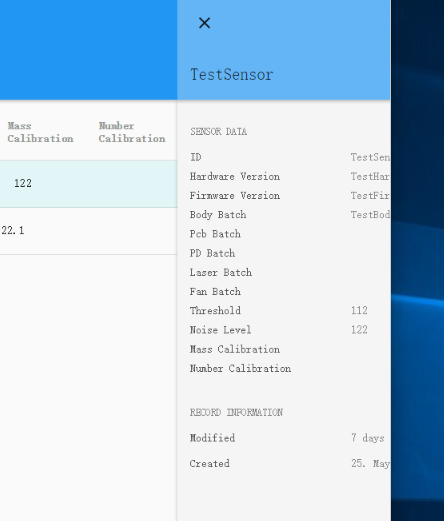
\includegraphics[width=0.5\textwidth]{before_responsive_edit.png}
 \bicaption[fig:before_responsive_edit]{响应式之前编辑页面超过屏幕宽度}{响应式之前编辑页面超过屏幕宽度}{Fig}{Edit page beyond screen width before responsive}
\end{figure}

因此,在客户端模型定义中引入了一个响应式的设计,首先属性定义会有一个可选的显示优先级(displayPriority)选项,其次模型视图群组接收一个狭窄模式(narrow-mode)的属性。如果某个字段的显示优先级为低级('low'),该字段对应的列表头和内容就会被加上一个CSS类:hide-in-narrow,如代码4.7所示,外面套了一层Media Query让元素在屏幕宽度低于1200像素的时候自动隐藏;同时因为CSS不能自动检测出来右边的编辑或详情页面是否打开,所以主动传入当前APP是否在一个详情路由(inDetailState)作为狭窄模式,模型视图群组会通过一个叫showProp的函数来判断是否显示该字段,如代码4.8所示。最终实现的效果如上文中图4-8所示,一些不太重要的属性在列表中被隐藏了。
\begin{lstlisting}[language={CSS}, caption={CSS类hide-in-narrow的代码}]
@media screen and (max-width: 1200px) {
  .hide-in-narrow {
    display: none;
  }
}
\end{lstlisting}

\begin{lstlisting}[language={JavaScript}, caption={传感器列表页面中的模型输入群组代码}]
function showProp(propDef) {
  return !scope.narrowMode || propDef.displayPriority !== 'low';
}
\end{lstlisting}
\subsection{代码生成器}
本模块不得不提的一点是使用了代码生成器generator-material-app,除了一开始的基础框架是自动生成的之外,还有一系列的子生成器,用于生成各种常用类型的Angular模块,极大地解放了开发人员也就是论文作者的生产力,基本只需要关注核心业务逻辑的编写。上文中提到的所有关于本模块的设计都是先用子生成器生成对应的Angular模块,在本模块中试验测试通过后,最后都反哺到了代码生成器中,所以核心业务逻辑基本只剩下前端和后端的模型定义了,这进一步解放了开发人员的生产力,因此本文作者也成为了该代码生成器的主要代码贡献者之一。主要常用的子生成器有:
\begin{description}
  \item[api name] 用于生成一个名为name的资源的后端API框架;
  \item[apiroute name] 用于生成一个名为name的资源前端API路由;
  \item[route name] 用于生成一个名为name的路由,路由更多地是包含在apiroute中被生成;
  \item[controller name] 用于生成一个名为name的控制器,控制器更多地是包含在apiroute中被生成;
  \item[directive name] 用于生成Angular可重用组件directive,如模型输入群组和模型视图群组就是先用这个生成再实现具体逻辑的;
  \item[factory name] 用于生成Angular服务factory,如模型定义服务就是先用这个生成再实现具体逻辑的;
  \item[service name] 用于生成Angular服务service,Angular服务的一种,没有必要在此赘述;
  \item[provider name] 用于生成Angular服务provider,Angular服务的一种,没有必要在此赘述;
  \item[decorator name] 用于生成Angular修饰器,是用于修改其他Angular库的行为的一种Angular模块;
  \item[filter name] 用于生成Angular过滤器,相当于一种转化函数,主要用在Angular的HTML代码中把一个值转换一种显示方式,比如在一些时间格式的显示,也可以直接在JavaScript代码中使用;
\end{description}
如图4-11所示,这是代码生成器在生成App和一个apiroute时的命令行交互界面:

\begin{figure}[!htp]
 \centering
 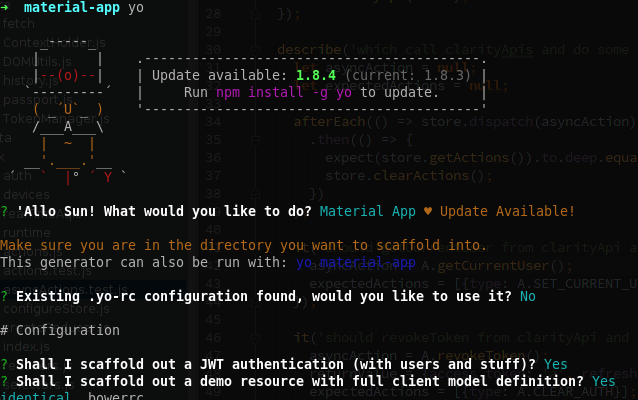
\includegraphics[width=0.8\textwidth]{generator_app.png}
 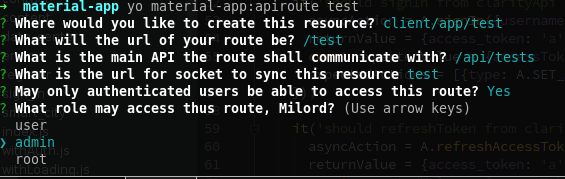
\includegraphics[width=0.8\textwidth]{generator_apiroute.png}
 \bicaption[fig:generator_cmd]{代码生成器命令行交互界面}{代码生成器命令行交互界面}{Fig}{Cmd ui of code-generator}
\end{figure}

\subsection{Git提交记录}
如图4-12和4-13所示,这是本文作者(git用户名为stupidisum)在本模块balanar和代码生成器generato-material-app这两个项目中的贡献记录。其中balanar因为部署需要,包含了一些第三方库的源代码,因此看起来行数比较多,但从提交数量上来比较,可以看出本模块与代码生成器的开发量比大概在5:3,基本上只要本模块中需要什么新的特性,在balanar中的一个资源上试验通过后,都会反过来加到代码生成器中,然后再用代码生成器重新生成其他资源对应的代码,从而减少了重复的开发工作。如果没有代码生成器,估计balanar中的提交数量要翻个三倍以上。
\begin{figure}[!htp]
 \centering
 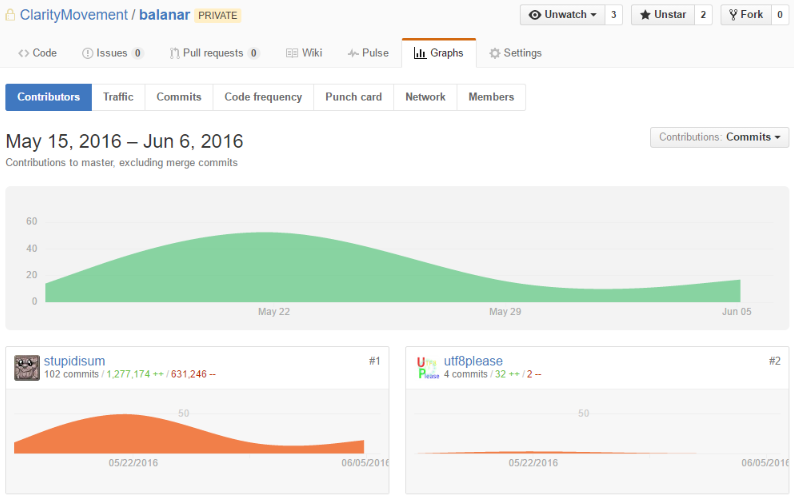
\includegraphics[width=\textwidth]{balanar_git.png}
 \bicaption[fig:balanar_git]{版本管理模块Git贡献记录}{版本管理模块Git贡献记录}{Fig}{Contributions to balanar}
\end{figure}
\begin{figure}[H]
 \centering
 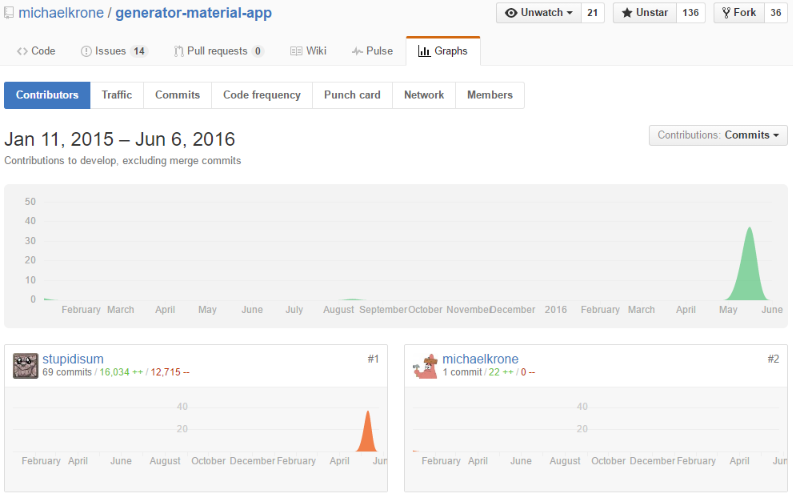
\includegraphics[width=\textwidth]{generator_git.png}
 \bicaption[fig:generator_git]{代码生成器Git贡献记录}{代码生成器Git贡献记录}{Fig}{Contributions to generator-material-app}
\end{figure}

\section{Smart Home 和 Smart City模块}
Smart Home和Smart City两个模块(下面以本模块代指这两个模块)架构相同,使用了现在越来越流行的灵活技术栈:React+Koa+MongoDB+RedisDB,其中React和Koa都是核心精简类型的,因此搭配有许多其他的库来完善各自的功能。所以React部分架构又可分为专注路由的react-router库、专注flux数据流的redux库和专注下一代浏览器Fetch标准\footnote{\url{https://fetch.spec.whatwg.org/}}的fetch库等,Koa部分架构又可分为专注路由的koa-router库、专注权限校验的koa-oauth-server库、专注MongoDB数据资源建模的Mongoose库和专注RedisDB缓存操作的redis库等。本模块是用ES6\footnote{ECMAScript 6,目前稳定的新版本的JavaScript}编写的,因此使用了Eslint来做语义上的代码风格检查;在构建工具方面,后端使用的依然是成熟且简单的gulp,但在前端使用了npm作为一个尝试。

下面将主要以权限校验为例,按照一次访问的生命周期的时间顺序,从服务端渲染、前端路由器、Redux数据流、API请求库和后端路由和数据模型等角度来介绍本模块的详细设计与开发。虽然从直观上看,用户是先访问前端页面再访问后端API,但其实用户从浏览器进入一个WEB应用,发生的第一件事是向服务器请求HTML文件,服务端渲染就发生在这个时候。最终介绍了一下主要组件的详细设计与开发。
\subsection{服务端渲染}
服务端渲染,如之前理论介绍中所讲,会在服务端把应用的HTML、JavaScript和CSS渲染成用户浏览器可以直接渲染的HTML页面,而原本选择渲染哪些HTML、JavaScript和CSS的是前端路由器,显然再实现一个前端路由器很不明智,所以服务端渲染还是利用前端路由器来选择路由的。

目前流行的服务端渲染方式是使用cookie,在渲染之前就获得了用户的token\footnote{令牌,包括访问令牌和刷新令牌,在前文的Oauth和JWT理论小节有过介绍},并把这个token传入前端路由器,前端路由器在分配路由之前会验证用户是否已经登录,决定是直接渲染目标路由(当前用户想要访问的页面)还是渲染隐式跳转(implicit redirect)后的登录路由(登录页面)。出于安全性的考虑,本模块不使用cookie,所以在渲染之前无法获得用户token,这就意味着这个首次访问的服务端渲染不会验证用户是否已经登录,本模块设计的服务端渲染是假设用户已经登录直接渲染出附加了一层加载蒙版的目标路由给客户端,在客户端加载完成之后,也就是已经获得存在客户端本地的token之后,再向服务器验证是否已经登录,如果是,则去掉加载蒙版,如果不是,则显式跳转(explicit redirect)到登陆路由。

如代码4.9所示,使用ReactDOM的renderToString函数把路由器成一个字符串,在通过一个template函数把渲染结果插入到index.html中并返回给客户端。如果是用流行的那种服务端渲染,store中除了现在的推送服务器,应该还包含用户token。
\begin{lstlisting}[language={JavaScript}, caption={服务端渲染样例代码}]
// ... 省去了错误处理部分,和一些声明无关的代码
// store是flux中的一个概念,redux中全应用只有一个store
const store = configureStore(memoryHistory);
// 只有服务端可以通过当前环境变量知道应该链接哪个推送服务器
store.dispatch(setRuntimeVariable({
  name: 'PUSH_SERVER',
  value: PUSH_SERVER,
}));
// ...
match({ routes, location: req.url }, (error, redirectLocation, renderProps) => {
  // ...
  // 给应用传递一些上下文环境
  const context = {
    store,
    // ...
  };

  // 用于让Material UI知道当前的浏览器类型
  const muiTheme = getMuiTheme({userAgent: req.headers['user-agent']});
  data.body = ReactDOM.renderToString(
    <MuiThemeProvider muiTheme={muiTheme}>
      <ContextHolder context={context}>
        <RouterContext {...renderProps} />
      </ContextHolder>
    </MuiThemeProvider>
  );

  // ...
  // 返回index.html
  res.send(template(data));
});
\end{lstlisting}

\subsection{前端路由器}
在前端渲染中,前端路由器通过一组用户自定义的路由声明来组建一个路由树,然后通过监听地址栏的变化,把路由器选择的路由上的对应组件嵌套起来渲染到对应的DOM对象上。

声明路由这一功能由react-router封装地非常完美,如代码4.10所示,这是Smart City模块的路由声明。一个路由的component属性里面传入的就是一个具体的组件,其中被withAuth包裹的SmartCity和DataCenter组件需要用户登录才能访问。如代码4.11所示,前端渲染在监听到地址栏变化后,会调用ReactDOM的render函数把路由器渲染到应用容器(appContainer)中。如果访问的是登录页面,那么经过路由器的选择,相当于渲染了如代码4.12所示的一个组件树。
\begin{lstlisting}[language={JavaScript}, caption={Smart City路由声明}]
<Route>
  <Route path="/" component={App} >
    <IndexRoute component={withAuth(SmartCity)}  />
    <Route path="sign_in" component={SignIn} />
    <Route path="contact" component={Contact} />
    <Route path="data_center" component={withAuth(DataCenter)} />
    <Route path="error" component={ErrorPage} />
  </Route>
  <Route path="*" component={NotFoundPage} />
</Route>
\end{lstlisting}
\begin{lstlisting}[language={JavaScript}, caption={Smart City前端渲染}]
history.listen(location => {
  // ...
  ReactDOM.render(
    <MuiThemeProvider muiTheme={muiTheme}>
      <ContextHolder context={context}>
        <Router history={history}>{routes}</Router>
      </ContextHolder>
    </MuiThemeProvider>,
    appContainer
  );
});
\end{lstlisting}
\begin{lstlisting}[language={JavaScript}, caption={Smart City登录页面实际渲染的组件树}]
<MuiThemeProvider muiTheme={muiTheme}>
  <ContextHolder context={context}>
    <App>
      <SignIn />
    </App>
  </ContextHolder>
</MuiThemeProvider>
\end{lstlisting}

如代码4.13所示,withAuth是一个React的高阶组件函数\footnote{HOC函数,higher-order component},可以把普通的组件变成有登录验证功能的组件。其中withLoading是另一个高阶组件函数,其功能是简单地把一个loading画面遮在当前Component上方,使其不能被用户操作,在此不予详述。withAuth函数接受一个组件,返回一个新定义的组件,这是HOC的标准格式。返回之前用redux的一个HOC函数connect包装了一下,后面会详细介绍。其核心逻辑在类里面。

\begin{lstlisting}[language={JavaScript}, caption={withAuth高阶组件函数}]
function withAuth(Component) {
  const ComponentWithLoading = withLoading(Component);

  class ComponentWithAuth extends React.Component {
    state = {
      waitingForAuth: true
    };

    componentWillMount = () => {
      if (this.props.location.action !== 'POP') {
        this.state.waitingForAuth = false;
      }
    };

    componentDidMount = () => {
      if (this.state.waitingForAuth) {
        this.props.onGetCurrentUser();
      } else {
        this.checkAuth();
      }
    };

    componentWillReceiveProps = this.checkAuth;

    checkAuth() {
      const {userSignedIn, location} = this.props;
      if (!userSignedIn && !this.state.waitingForAuth) {
        this.props.onPush({pathname: '/sign_in', state: {next: location}});
      }
    }

    render = () => this.props.userSignedIn ? <Component /> : <ComponentWithLoading />;
  }

  const mapStateToProps = state => ({userSignedIn: isUserSignedIn(state)});
  const mapDispatchToProps = dispatchMapper({push, getCurrentUser});

  return connect(mapStateToProps, mapDispatchToProps)(ComponentWithAuth);
}
\end{lstlisting}

完整的前端权限校验流程是这样的:
\begin{description}
  \item[步骤零] 路由控制,如果是需要权限的路由跳到步骤一,如果是登录路由,跳到步骤四,否则跳到步骤五。
  \item[步骤一] 检查是否为首次渲染,如果是跳到步骤二,如果不是直接跳到步骤三。具体表现为检查当前访问(location)是不是直接进来的(action为'POP'),如果是应用内页面跳转的话,action是'PUSH'。
  \item[步骤二] 获取当前用户信息,完成后之后跳到步骤三。具体表现为调用了onGetCurrentUser函数,该函数是redux的一个action,完成后会触发下一个周期的componentWillReceiveProps,也就是checkAuth函数,至于如何触发的将在下一个小节Redux数据流中介绍。
  \item[步骤三] 检查当前用户是否拥有足够权限,如果没有跳到步骤四,如果有直接跳到步骤五。具体表现为调用了checkAuth函数,跳转到登录页面时会把当前地址存储在登录location的状态中作为登录后跳转的下一个地址(state: {next: location})。
  \item[步骤四] 用户登录并自动跳转,跳到步骤零。具体表现为调用了如代码4.14所示的SignIn组件的onSubmit函数被触发,跳转到之前指定的下一个地址(next),或者缺省的主页('/')。
  \item[步骤五] 目标路由正常显示。
\end{description}
\begin{lstlisting}[language={JavaScript}, caption={SignIn组件中的onSubmit函数}]
onSubmit = model => {
  const locationState = this.props.location.state || {next: '/'};
  this.props.onSignIn(model)
    .then(this.props.onGetCurrentUser)
    .then(() => this.context.router.replace(locationState.next || '/'))
}
\end{lstlisting}
\subsection{Redux数据流}
Redux是Flux的一个变种,大部分行为和Flux相同,如图4-14,某个地方把Action(行为)传入Dispatcher(触发器),会引起Store(仓库)的变化,Store的变化又会引起View(视图)的变化,视图中可以反过来用Callback(回调)函数再把Action传给Dispatcher。
\begin{figure}[!htp]
 \centering
 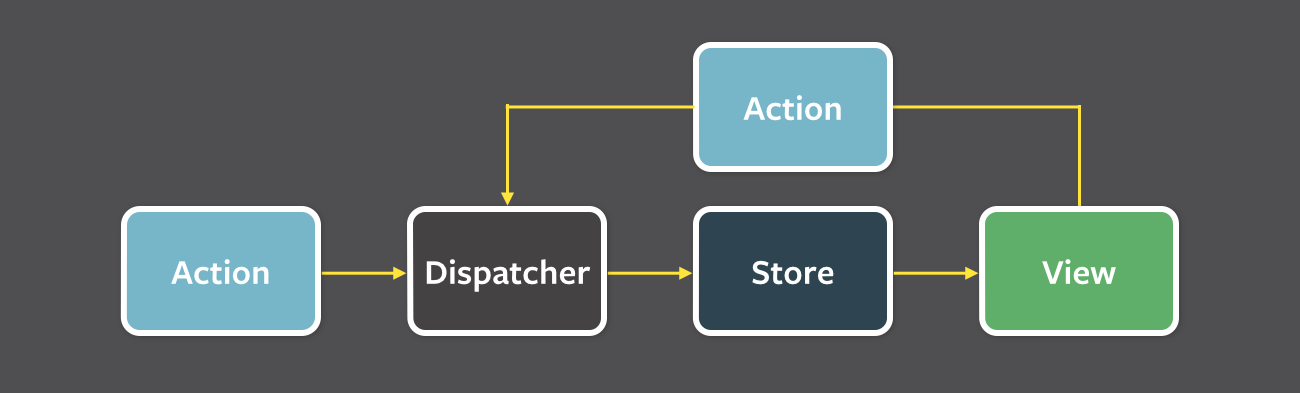
\includegraphics[width=0.9\textwidth]{flux.png}
 \bicaption[fig:flux_data_flow2]{Flux 数据流}{Flux 数据流}{Fig}{Flux Data Flow}
\end{figure}

\begin{figure}[!htp]
 \centering
 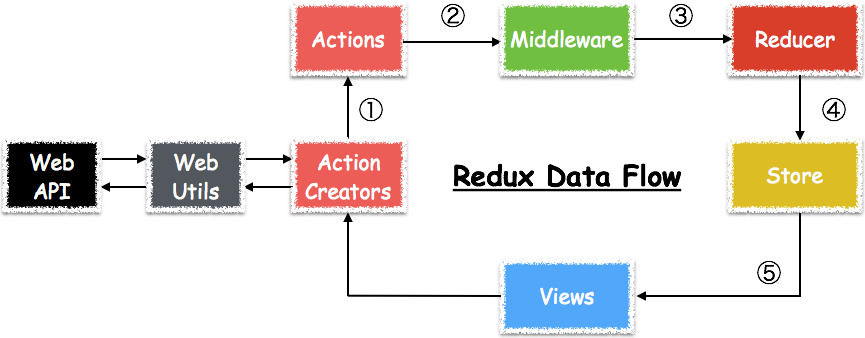
\includegraphics[width=0.9\textwidth]{redux.jpg}
 \bicaption[fig:redux_data_flow]{Redux 数据流}{Redux 数据流}{Fig}{Redux Data Flow}
\end{figure}

如图4-15,Redux把Flux中的Action扩展为Action Creators(行为构造器)、Actions两个步骤并提供了一个dispatch(触发)函数来触发一个Action,把Flux中的Dispatcher细分为Middlewares(中间件)和Reducer(处理器或直译为压缩器)两个步骤,Redux把Action定义为一个含有两个属性的对象,分别是type和value,type的值就是Action Types(行为类型),把Store中实际存储的状态树叫做State,Redux的特点在于
\begin{enumerate*}
  \item 整个应用只有一个Store
  \item 函数式编程,Reducer应当是纯函数,没有任何副作用
  \item 状态不可修改,Reducer中不可以修改State变量,而是每次都必须返回一个新的完整的State变量
\end{enumerate*}。Redux推荐使用State的第一层属性来表示应用所需要的不同状态,对于第一层的每个属性都定义一个SubReducer(子处理器)函数,最后使用它提供的combineReducer(整合处理器)函数组合起来成为图中的Reducer,SubReducer应当接收一个缺省为initialState(初始状态)的previousState(旧的状态),返回一个nextState(新的状态)。Redux不推荐直接手动构造一个Action,所以一般会专门定义一种Action Creator(行为构造器)函数。如果构造Action之前需要进行一些异步操作再返回这个新的Action,比如需要调用Web Utils函数来调用Web API拿到结果后使用结果来构造Action,一般会专门定义一种特殊的Action Creator叫做Async Action Creator(异步行为构造器)。如果一个行为不仅仅要改变某个状态,还有一些额外副作用的操作的话,Redux推荐放在Middleware中,不推荐放在Action Creator和Reducer函数中,Action Creator和Reducer函数都应该只负责一件事。

如果是跟React一起使用,想要让一个React Component(React组件)得到State来改变视图、能够注册callback来dispatch(action),就得用到Redux的一个重要函数connect(连接),它的作用就是把store中的state和某一个Component联系起来。connect的第一个参数是mapStateToProps(把状态映射到组件属性),虽然这里是map\emph{\textbf{State}}ToProps而不是map\emph{\textbf{StatePartials}}ToProps,但Redux推荐的是只取需要的部分映射到Component的属性上,而不是把整个State暴露给Component;如果当前Component需要的属性不是State树中直接存在的某个节点,那么一般会专门定义一种Selector函数来对State进行一些操作后返回Component需要的属性。connect的第二个参数是mapDispatchToProps(把触发函数映射到组件属性),虽然这里为了保持灵活度,是map\emph{\textbf{Dispatch}}ToProps而不是map\emph{\textbf{DispatchCallback}}ToProps,但Redux还是推荐使用构造一些callback传给Component,而不是直接把dispatch直接扔给Component。

如图4-16所示,分别是azwraith和robotic的redux目录结构,其中开发robotic时,本文作者对其理解还不够深入,所以结构比较粗糙。State的第一层属性对应不同的文件夹如auth、devices等;SubReducer函数分别定义在文件夹中的reducer.js中;一个State对应的Action Types和Action Creators函数(包括异步的)定义在文件夹中的actions.js中;Selector函数定义在selectors.js中。根目录下的actions.js用于把所有第一层属性的Actions Creators组合起来方便引用,reducers.js的作用是把所有reducer函数组合成一个rootReducer,configStore.js提供一个配置函数让客户端和服务端第一次载入时能够构造出一个新的Store。createReducer.js中的createReducer函数和index.js中的dispatchMapper函数是本模块自定义的两个函数,用于简化代码量,增加可读性,createReducer用于使用简单的Map(在这里是一个JavaScript对象,以映射形式表示一组有名字的函数)来构造Reducer,dispatchMapper用于使用简单的Map来构造一组callback。
\begin{figure}[!htp]
 \centering
 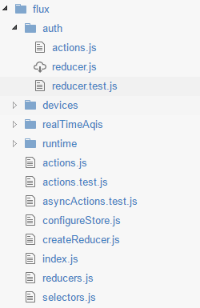
\includegraphics[width=0.4\textwidth]{redux_dir.png}
  \hspace{1cm}
 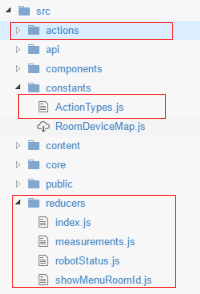
\includegraphics[width=0.4\textwidth]{robotic_redux_dir.png}
 \bicaption[fig:robotic_redux_dir]{Smart City和Smart Home模块redux目录结构}{Smart City和Smart Home模块redux目录结构}{Fig}{Redux directories of Smart Home and Smart City}
\end{figure}

如代码4.15所示,在这里主要以azwraith为例介绍首次访问一个受保护的路由(Route with auth)的过程中Redux的数据流是怎样的:
\begin{enumerate}
  \item 一旦有状态改变(包括初始状态),connect函数使用isUserSignedIn把userSignedIn这样的信息映射给了ComponentWithAuth,使用了dispatchMapper函数把push和getCurrentUser变成了onPush和onGetCurrentUser这两个callback函数映射给Component;
  \item ComponentWithAuth在遇到首次访问受保护的路由的情况下会先调用onGetCurrentUser函数,即getCurrentUser;
  \item getCurrentUser会调用clarityApi.getCurrentUser向服务器请求当前用户;
  \item 请求无论成功或失败后都会调用setCurrentUser这个Action Creator并dispatch它返回的Action;
  \item 如果有注册Middleware,dispatch会先把dispatch函数本身和这个Action传给socketIoMiddleware这样的Middleware;
  \item socketIoMiddleware中又会调用dispatch(代码中为next),重复上一步骤直到没有Middleware了;
  \item dispatch会把当前状态和这个Action交给Reducer,Reducer又会把它们传递给auth对应的用createReducer构造的SubReducer;
  \item 最终store会使用Reducer返回的结果更新自己的State,又回到第1步,只不过这次会通过权限验证或者跳转到登陆路由;
\end{enumerate}
\begin{lstlisting}[language={JavaScript}, caption={Smart City模块权限校验Redux数据流相关代码}]
/* 在withAuth.js 中  */

// push其实是一个react-router被整合到Redux中之后的一个Action Creator
import { push } from 'react-router-redux';

function withAuth(Component) {
  // ...
  const mapStateToProps = state => ({userSignedIn: isUserSignedIn(state)});
  const mapDispatchToProps = dispatchMapper({push, getCurrentUser});

  return connect(mapStateToProps, mapDispatchToProps)(ComponentWithAuth);
}

/* 在auth/actions.js中  */

// clarityApi将在下一小节前端API库中介绍;
import * as clarityApi from '../../clarityApi';
// Action Types
export const SET_CURRENT_USER = 'SET_CURRENT_USER';

// Action Creators
export const setCurrentUser = value => ({type: SET_CURRENT_USER, value});

// Async Action Creators
export function getCurrentUser() {
  return dispatch => clarityApi.getCurrentUser()
    .then(user => dispatch(setCurrentUser(user)))
    .catch(() => dispatch(setCurrentUser({})));
}

/* 在selectors.js中 */

// 从state中筛选出返回用户是否已经登录这样的信息
export const isUserSignedIn = state => {
  const currentUser = state.auth.currentUser;
  return currentUser && currentUser.email;
};

/* 在index.js中  */

// dispatchMapper函数就是简单地把一个的Action Creators组成的Map,
// 变成一个接受dispatch为参数的并返回一个由callback组成的Map的函数,
// 这些callback的名字以on开头加上原本Action creators大写首字母的名字
export function dispatchMapper(actionCreators) {
  return dispatch => {
    const map = {};
    Object.keys(actionCreators).forEach(name => {
      const onActionCreator = 'on' + name.charAt(0).toUpperCase() + name.slice(1);
      map[onActionCreator] = (...params) => dispatch(actionCreators[name](...params));
    });

    return map;
  };
};

/* 在auth/reducer.js中 */

export default createReducer({}, {
  [A.SET_CURRENT_USER]: (auth, {value}) => ({...auth, currentUser: value}),
});

/* 在createReducer.js*/

// createReducer函数的作用是把一个初始状态和一个针对每个Action Type的处理函数组成的Map,
// 变成一个正常的SubReducer;
export default function createReducer(initialState, handlers) {
  return (state = initialState, action) => {
    const handler = (action && action.type) ? handlers[action.type] : undefined;

    if (!handler) {
      return state;
    }

    return handler(state, action);
  };
}

/* 在另外的../data/socket.js中 */

// socketIoMiddleware是一个监听权限验证Action来重连socket的中间件,
// socket.io部分的的权限验证在前文的理论中已经介绍过,这里只是实现了一下。
export const socketIoMiddleware = () => next => action => {
  const res = next(action);
  if (!socket) return res;
  switch (action.type) {
    case A.SET_CURRENT_USER: {
      if (socket.connected) socket.disconnect();
      socket.connect();
      break;
    }
  }
  return res;
};
\end{lstlisting}
\subsection{API请求库和WebSocket}
因为fetch是一个比较底层的库,本模块在fetch库的基础上封装了一层clarityFetch的WEB API库。为了方便前端在Component和Redux中调用API,本模块在clarityFetch基础上又封装了一个叫clarityApi的WEB Utils库,有像getCurrentUser、getRoboticStatus(是在Smart Home模块中使用的)这样的简单函数。但本模块使用了Oauth做权限校验,所以clarityFetc需要使用Redux中才有的一些信息和函数,如访问令牌等,由于Redux部分已经依赖了clarityApi,间接依赖了clarityFetch,所以这里引入了一个TokenManager来防止循环依赖,Redux部分在configStore时把获取这类信息的函数以回调函数的形式传入TokenManager,clarityFetch再调用TokenManager来获得Redux中才有的信息和函数,但其实clarityFetch并不知情这些信息来自于Redux。

clarityFetch主要有以下这些特性:
\begin{enumerate}
  \item 默认选项的配置,比如说默认接收类型(Acceppt)application/json格式
  \item 允许url为对象从而可以传递参数
  \item 使用快捷的post、delete等方法省去指定请求类型
  \item 在每个请求的header中附加当前用户的访问令牌,访问令牌由自定义的TokenManager的getAccessToken方法获得
  \item 在发请求(request)之前如果请求类型(Content-Type)是application/json,对请求的body做了JSON序列化;
  \item 在接收到回应(response)之后,增加了统一的错误处理,如果错误原因是访问令牌不合法,会使用TokenManager的refreshToken方法尝试刷新一下访问令牌,然后再用新的访问令牌重发本次请求,期间一旦发生错误就像普通的错误请求一样抛出原本的错误异常;
  \item 在接收到成功的回应之后,如果接收类型(Acceppt)是application/json,对回应的body做了JSON反序列化;
\end{enumerate}

\subsection{后端路由器和数据模型}
后端路由器使用了koa-router和koa-oauth-server两个库,如代码4.16所示,在控制器的构造函数中加入一行代码就可以让在其后注册的API需要权限验证,而之前的不需要。
\begin{lstlisting}[language={JavaScript}, caption={Smart City和Smart Home模块后端权限控制相关代码}]
/* 在routes.js中 */
loadRoutes(api, '/v2/users', require('./user/controller').default);

/* 在user/controller.js中 */
import oauth from '../oauth';
import convert from 'koa-convert';
import User from '../../models/User';

export default (router) => {
  router.post('/', create);
  router.use(convert(oauth.authenticate()));
  router.get('/current', getCurrent);
}
async getCurrent(ctx) {
  ctx.body = ctx.state.oauth.token.user;
}
async create(ctx) {
  // ...
  const user = {
    email: ctx.request.body.email,
    password: ctx.request.body.password,
  };

  await User.register(user);
  // ...
}

/* 在oauth.js中 */
import OauthServer from 'koa-oauth-server';
import oauth from '../models/oauth';

export default new OauthServer({
  model: oauth,
});

/* 在models/oauth中 */

// 此oauth模型中的属性函数都是是OauthServer要求实现的
export default const oauth = {
  getAccessToken: ...,
  getRefreshToken: ...,
  getClient: ...,
  getUser: ...,
  saveToken: ...,
  revokeToken: ...,
  validateScope: ...,
  revokeAccessToken: ...,
}
\end{lstlisting}

如代码4.17所示,这里使用的User模型也和版本管理模块一样用的是Mongoose。
\begin{lstlisting}[language={JavaScript}, caption={Smart City和Smart Home模块后端User模型}]
/* 在models/User.js中 */
const User = mongoose.Schema({
  email: {type: String, unique: true, required: true},
  password: {type: String, required: true},
  ...
});

User.static('register', async function(userInfo) {
  const user = new this(userInfo);
  // validate before we begin to hash the password ans save to db
  await user.validate();
  await user.hashPassword();
  return await user.save();
});
\end{lstlisting}

\section{主要组件详细设计和开发}
本小节介绍本模块的主要组件,具体分为业务无关的通用组件,Smart City业务组件和Smart Home业务组件,整体上是从小到大的顺序,后面的组件实际使用或包含了前面的组件。
\subsection{业务无关的通用组件}
\subsubsection{Echart组件}
本模块使用百度开发的Echarts图表库来绘制图表,虽然国外有更好的highcharts和D3等图表库,但它们一个收费,一个过于高级,处理本模块简单的图表绘制需求不够经济适用。为了在React中更好地使用Echarts,本模块封装了一个业务无关的通用Echart组件。

Echarts中绘图的主要是需要一个固定高度和宽度的元素作为容器,然后靠一个配置项配置图表中的各类元素,通过传入回调函数来控制来自定义的交互,Echarts会以事件的的形式触发这些回调函数,所以本组件接收style、option和onEvents三个参数,分别用来让调用者可以控制Echart容器的宽高、配置项和回调。同时为了让Echarts图表能够自动适应屏幕宽度的变化,在React生命周期的componentDidUpdate函数中如果检测出容器高度或宽度变了,会重新调用调用Echarts的init函数。本组件在两个模块中共用,下文的AqiChart组件和HomePanel组件都使用了Echart组件来绘制折线图。实际效果如图4-17所示,手动改变高度和宽度后,Echart组件会自动适应。
\begin{figure}[!htp]
 \centering
 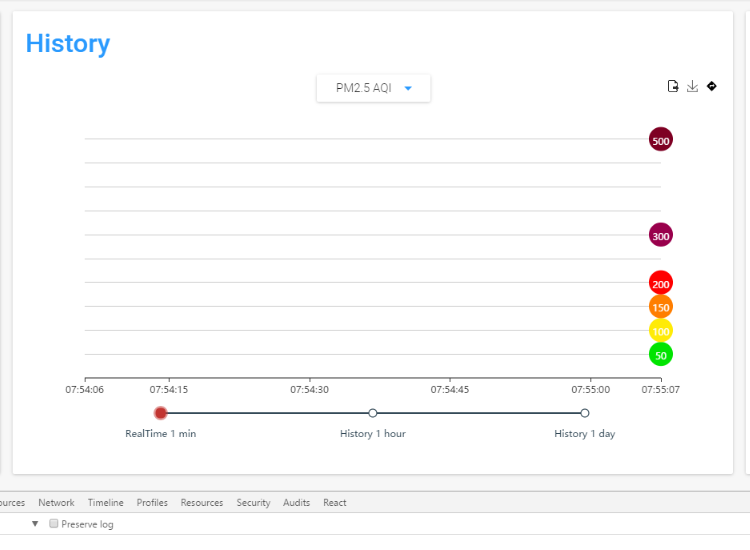
\includegraphics[width=0.45\textwidth]{echart1.png}
 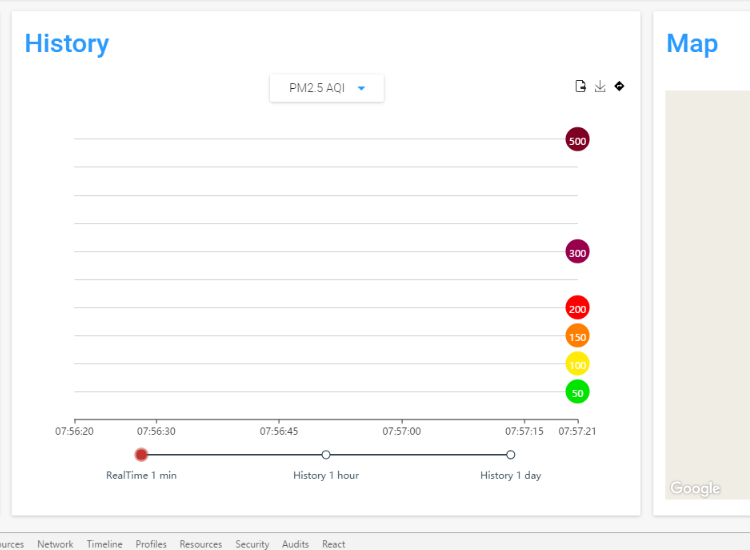
\includegraphics[width=0.45\textwidth]{echart2.png}
 \bicaption[fig:echart]{Echart组件自动适应}{Echart组件自动适应}{Fig}{Auto-sizing of Echart Component}
\end{figure}
\subsubsection{HorizontalAccordion组件}
因为Smart Home模块独特的设计风格,所以设计了HorizontalAccordion(水平手风琴)这样一个能够在水平方向像手风琴一样展开任意一片的通用组件。它的具体行为就是把自己包含的所有子组件(children components)都当做在手风琴叶片,任意一个叶片被点击,它就会让那个叶片展开,其他叶片收起,同时这个过程为了不给用户造成突兀的感觉增加了动画效果。。具体效果在这里先不演示了。
\subsubsection{Loading组件}
Loading组件就是上文在权限检验中提到的浮在普通页面上的loading页面,通过一个withLoading的高阶组件函数悬浮在一个等待验证授权的组件上方,实现效果如图4-20。
\begin{figure}[!htp]
 \centering
 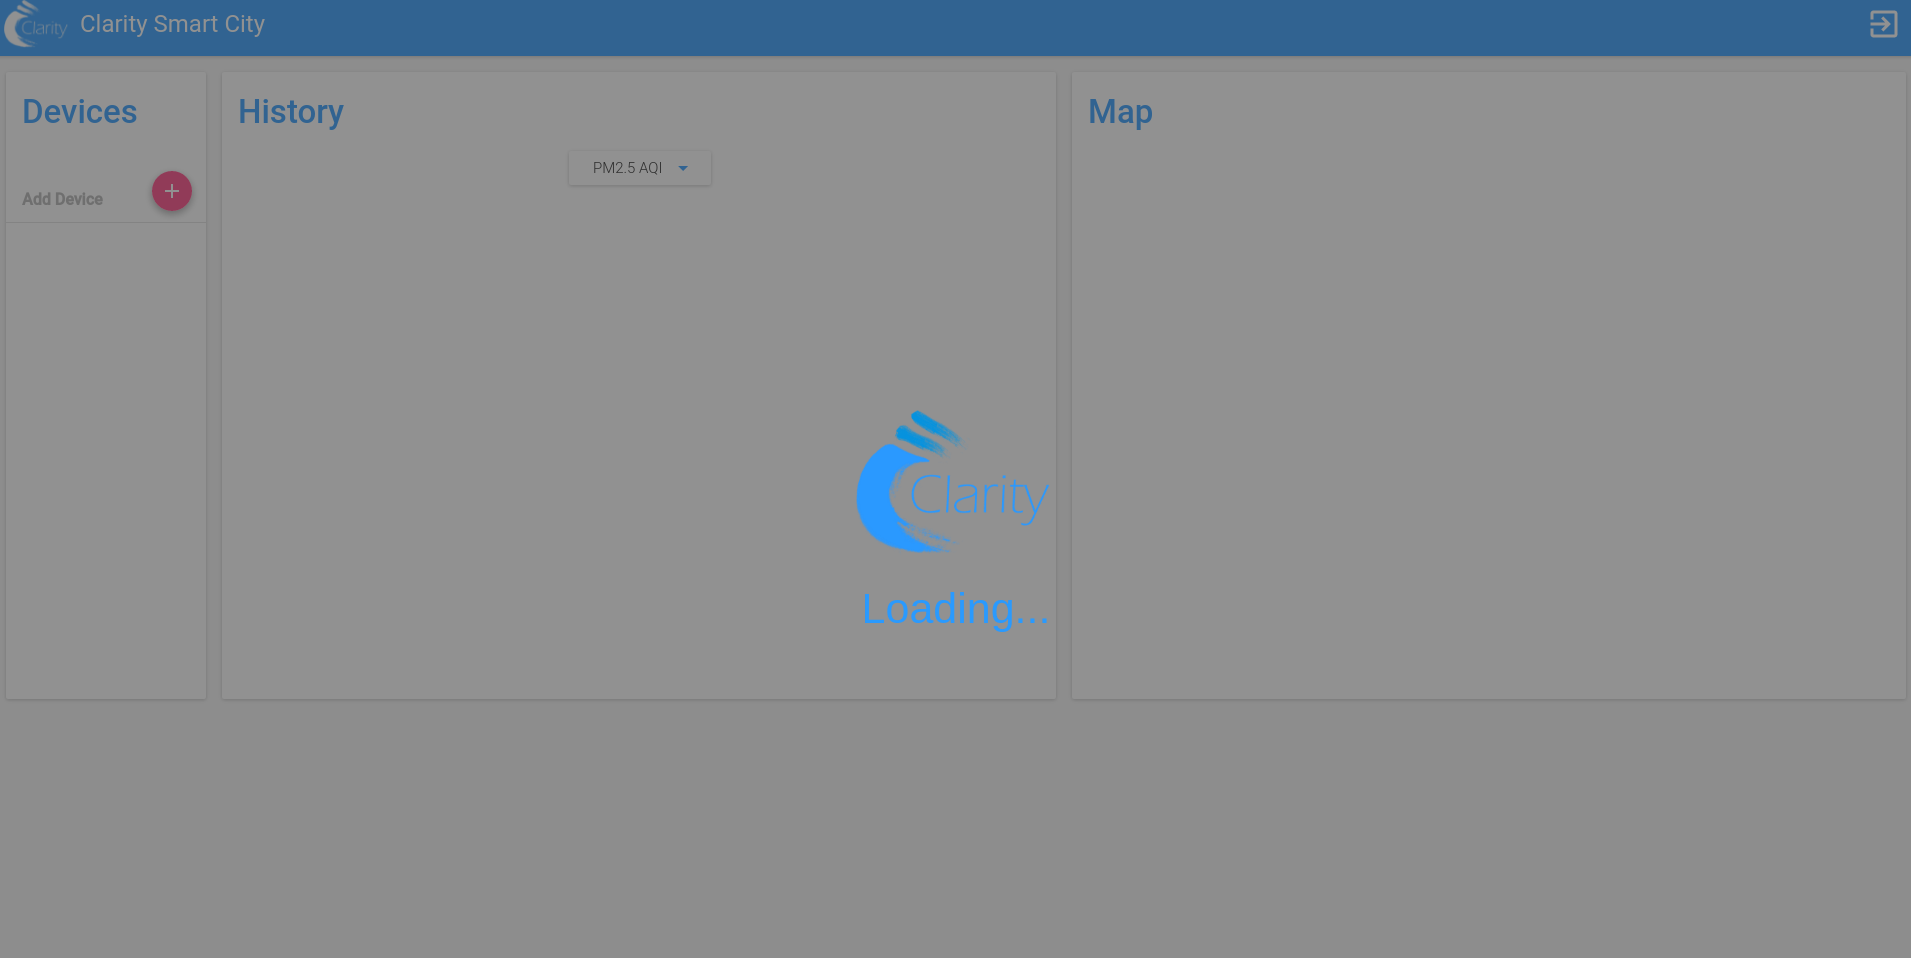
\includegraphics[width=\textwidth]{loading.png}
 \bicaption[fig:loading]{loading页面}{loading页面}{Fig}{Loading Modal}
\end{figure}
\subsection{Smart City业务组件}
\subsubsection{AqiChart组件}
Smart City模块需要把用户指定的设备的实时、每分钟和每小时空气质量数据用折线图的形式展示出来,同时折线图上的数据应当能够立即下载,因此本模块中定义了一个专门绘制历史空气质量折线图的AqiChart组件。因为实时数据是通过Socket.io更新的,AqiChart自己维护不太合适,所以它通过Redux数据流获取当前实时数据,它自己内部用计时器每小时和每分钟各获取一次相应时间间隔的历史数据。但AqiChart还需要外部决定显示哪些设备以及显示的度量类型,同时还需要外部传入给Echart用的样式,所以它接收devices、measurementType和style三个参数。在渲染时,AqiChart动态地生成“RealTime 1 min”(实时一分钟)、History 1 hour(历史一小时每分钟)和History 1 day(历史一天每小时)的三个的子配置项以及用于在Echart中选择三者之一的timeline(时间线)配置项,另外还生成toolbox(工具栏,包括导出到csv、保存为图片和高级下载三个功能)、title(标题)、legend(图例)、xAxis(x轴)、yAxis(y轴)等一系列配置项,最后组装到一起作为option参数,并且把需要监听的事件对应的回调函数构成onEvents参数以及外部传入的style一起传递给Echart组件。实现效果如图4-18所示
\begin{figure}[!htp]
 \centering
 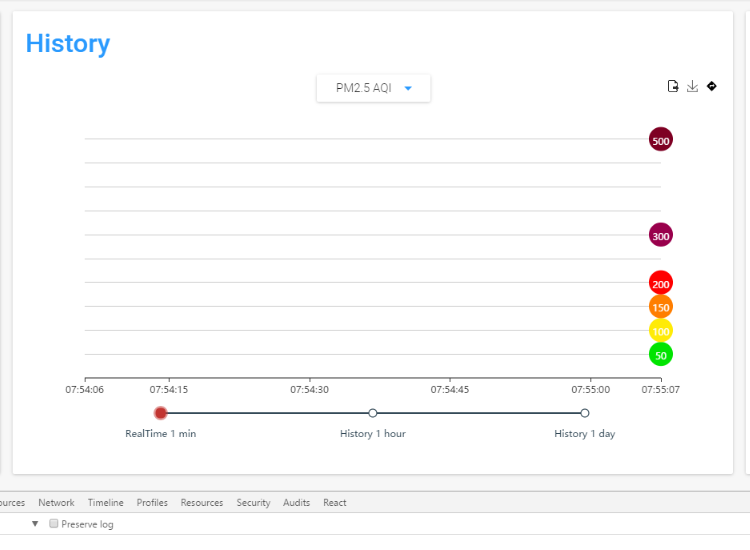
\includegraphics[width=0.45\textwidth]{echart1.png}
 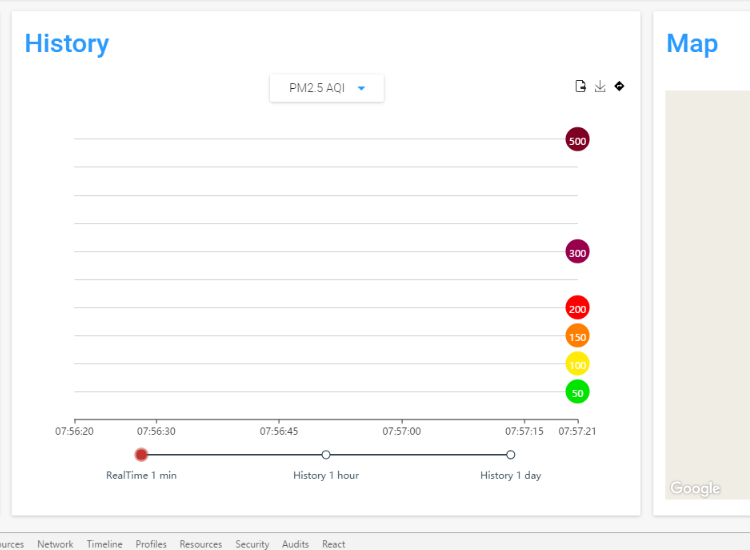
\includegraphics[width=0.45\textwidth]{echart2.png}
 \bicaption[fig:AqiChart]{Echart组件自动适应}{Echart组件自动适应}{Fig}{Auto-fit of Echart Component}
\end{figure}
\subsubsection{AqiMap组件}
Smart City模块需要绘制地图来实时展示设备的位置和当前空气质量,所以本模块封装了一个AqiMap组件,引用了一个叫google-map-react的开源库中的GoogleMap组件,使用Google地图来绘制地图。另外自定义了一个SensorMarker组件来在地图上用气泡标识传感器,鼠标悬浮在气泡上会显示传感器详细信息和实时数据,在实时数据的Redux数据流中加上了对传感器位置的更新,于是就做到了实时更新地图上设备的位置。按理说,这个GoogleMap组件应该像Echart组件那样自己适应容器大小,但是它没有实现这个功能,所以本组件又自己实现了自适应容器大小以及自动根据传感器位置找到合适中心点和缩放比例(Google地图定位需要的两个核心参数)的功能。如图4-19所示,原本中心在美国的地图,在增加了一个位置在非洲的设备后,自动变成了中心在大西洋,同时显示了两个设备。
\begin{figure}[!htp]
 \centering
 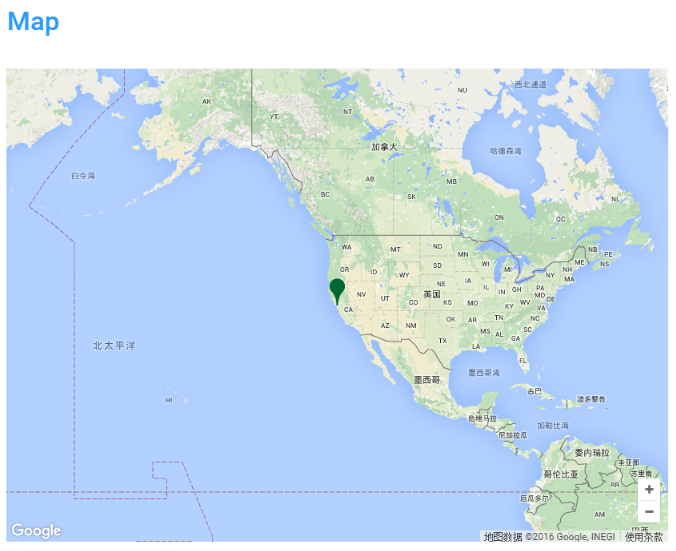
\includegraphics[width=0.45\textwidth]{AqiMap1.png}
 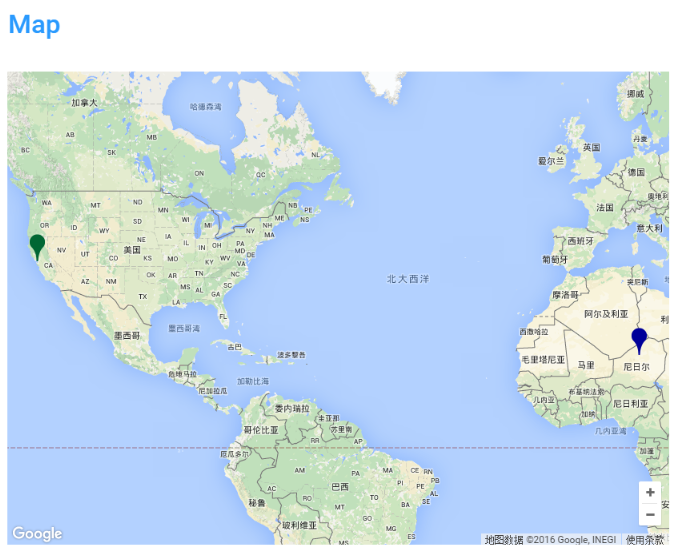
\includegraphics[width=0.45\textwidth]{AqiMap2.png}
 \bicaption[fig:AqiMap]{AqiMap组件自动适应}{AqiMap组件自动适应}{Fig}{Auto-sizing of AqiMap Component}
\end{figure}
\subsubsection{SmartCity组件}
SmartCity模块最为重要的一个路由组件就是SmartCity组件,SmartCity布局上分三个部分,左边是设备列表,有一个最小宽度,右边的宽度平分给一个AqiChart组件和一个AqiMap组件。设备列表中可以添加、删除、隐藏和显示设备,另外还用实线和虚线作为折线图的图例,用线的颜色表示不同的设备。这里之所以叫设备是因为有一个概念上的转移,最终用户并不需要了解这是传感器,只需要知道他拥有的智能设备能够检测空气质量就行。SmartCity组件在设备数组上附加上设备列表中的选中状态,然后传递给AqiChart和AqiMap来决定隐藏还是显示设备,选中状态不上传到服务器而是保存在本地。实现效果如图4-21所示。
\begin{figure}[!htp]
 \centering
 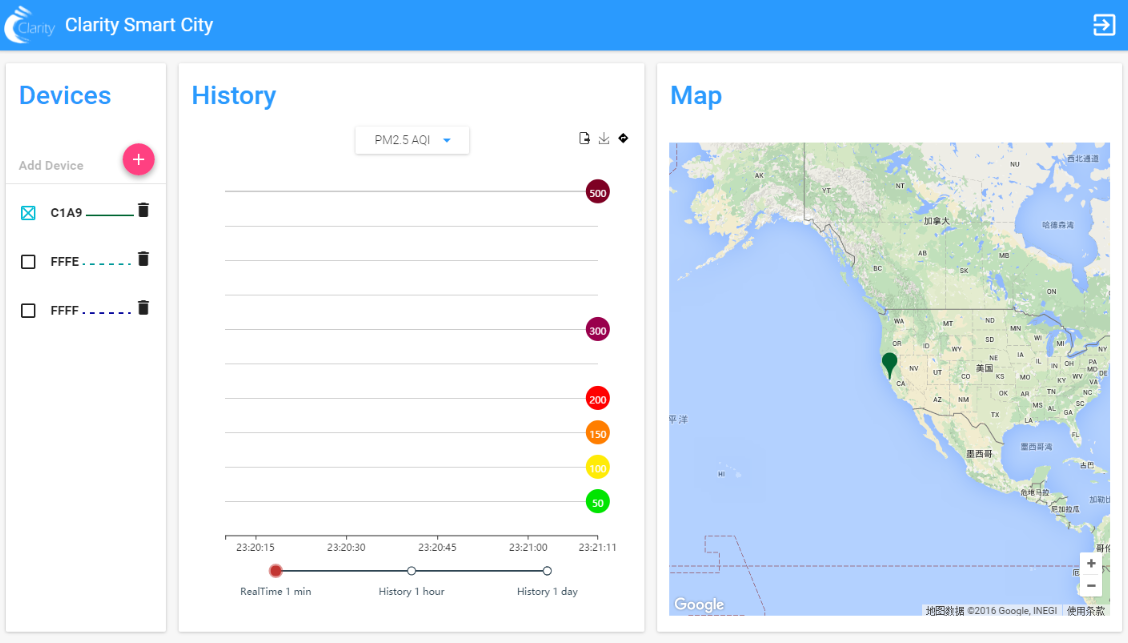
\includegraphics[width=\textwidth]{smart_city.png}
 \bicaption[fig:smart_city]{SmartCity组件}{SmartCity组件}{Fig}{SmartCity Component}
\end{figure}
\subsubsection{DataCenter组件}
数据是Clarity的一大财富,所以SmartCity模块专门开发了一个DataCenter路由组件用于专门做数据方面的事情,不过目前主要的功能就是高级下载。虽然AqiChart组件中的导出到csv功能,能够让用户“所见既所下”,但是受制于图表在时间跨度上难以让用户自己选择,所以另外开发了高级下载功能,让用户能够选择任意的时间跨度,当然还是选择设备、时间精度和空气质量度量的,只不过都是以表单的形式。

\subsection{Smart Home业务组件}
Smart Home中主要有三个业务组件PersonPanel、HomePanel和CityPanel,它们被放在一个水平手风琴中作为叶片,因为叶片有两种宽度,所以这些组件内部都有展开和收起两种模式。其中PersonPanel由于是需求优先级最低的一个,所以开发进度被搁置了,这里不予详细介绍。另外为了实现上文中所提到的智能家居解决方案,本模块还另外设计了Room和Robot两个组件。
\subsubsection{Room组件}
Room组件背景是动画风格的各种房间,点击后会出现一个菜单。如图4-22所示,需求要求直观的显示每个房间的空气质量情况,所以Room组件会在房间上面加一层窗帘状的灰雾,遮住的范围越大、透明度越低,表示房间空气质量越差。需求要求用户能够手动地控制机器人去某个房间,所以Room的菜单上面有个机器人图标的按钮,点击就是下令来净化当前房间。需求要求用户可以查看每个房间的实时空气质量,所以Room的菜单上还有一个列表图标的按钮,点击后弹出一个弹窗,其中包含一个用Echart组件绘制的实时数据折线图。
\begin{figure}[!htp]
 \centering
 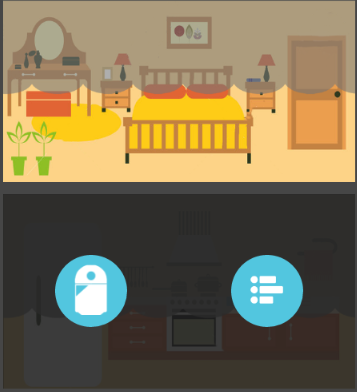
\includegraphics[width=0.6\textwidth]{rooms.png}
 \bicaption[fig:rooms]{Room组件}{Room组件}{Fig}{Room Component}
\end{figure}
\subsubsection{Robot组件}
\begin{figure}[!htp]
 \centering
 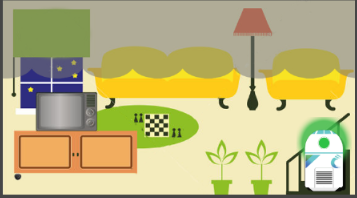
\includegraphics[width=0.6\textwidth]{robot_on.png}
 \bicaption[fig:robot_on]{正在净化房间的Robot组件}{正在净化房间的Robot组件}{Fig}{Robot Component purifying a room}
\end{figure}
Robot组件需要传入它能去的所有房间的位置信息,它自己有一个服务器实时推送的状态(实体机器人的状态),状态中包含机器人上次访问的房间、目的地房间、是否接通电源、空气净化器是否打开、是否处于手动模式、是否处于出错状态等信息,并根据它们来决定Robot的工作状态是否要切换到正在工作或者出错状态,分别会让Robot头部发绿光和红光。如果上次访问的房间和目的地房间不同,则Robot会向目的地房间移动(动画效果),由于不能得知机器人的移动进度,所以这个动画效果会越来越慢且不会到达指定位置,直到收到新的上次访问房间或者目的地房间。如图4-23所示,机器人正在净化一个空气状况不太良好的房间。
\subsubsection{HomePanel组件}
HomePanel组件是实现智能家居解决方案的主要业务组件,如图4-24所示,HomePanel背景是一个动画风格的蓝天白云二层小房子,有四个房间,其中三个各有一个Room组件,还有一个空房间放了一个选择手动还是自动模式的开关,右下角的房间里有一个Robot组件。如图4-25所示,在狭窄模式下,HomePanel会显示四个房间综合的空气质量和机器人的工作状态。
\begin{figure}[!htp]
 \centering
 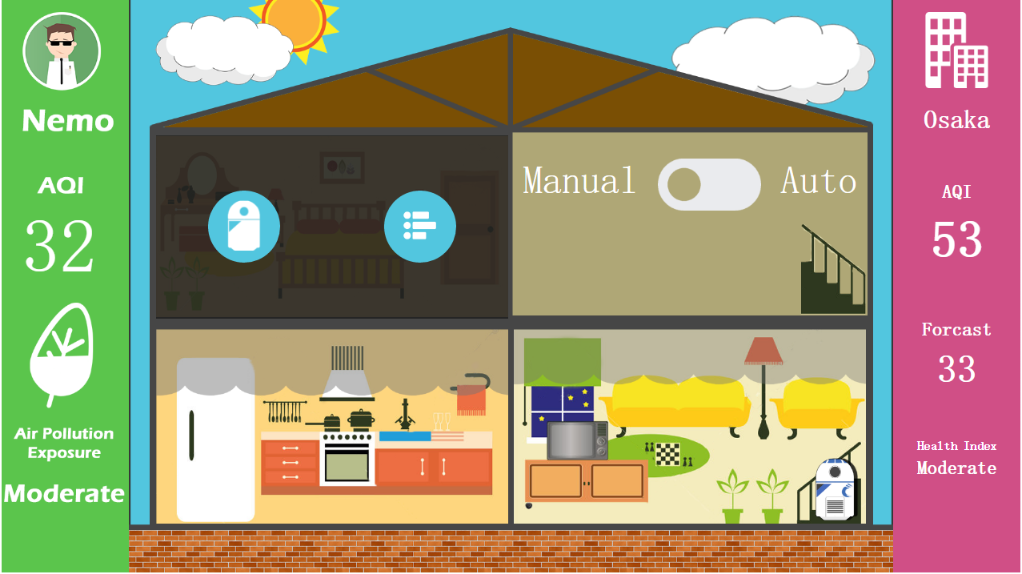
\includegraphics[width=\textwidth]{HomePanel.png}
 \bicaption[fig:HomePanel]{HomePanel组件}{HomePanel组件}{Fig}{HomePanel Component}
\end{figure}
\subsubsection{CityPanel组件}
CityPanel通过用户的浏览器定位用户的位置,然后显示其周围的空气质量热力图和当前城市的空气质量及预告,这里的空气质量热力图也有一个自定义的组件AirMap,与上面的AqiMap一样都使用了google-map-react库的GooleMap组件,不过地图上实际绘制的内容不同。如图4-25所示,这是当初项目初步完成在日本大阪给目标客户演示时的截图。如图4-24所示,在狭窄模式下CityPanel会显示只显示空气质量和预告。
\begin{figure}[!htp]
 \centering
 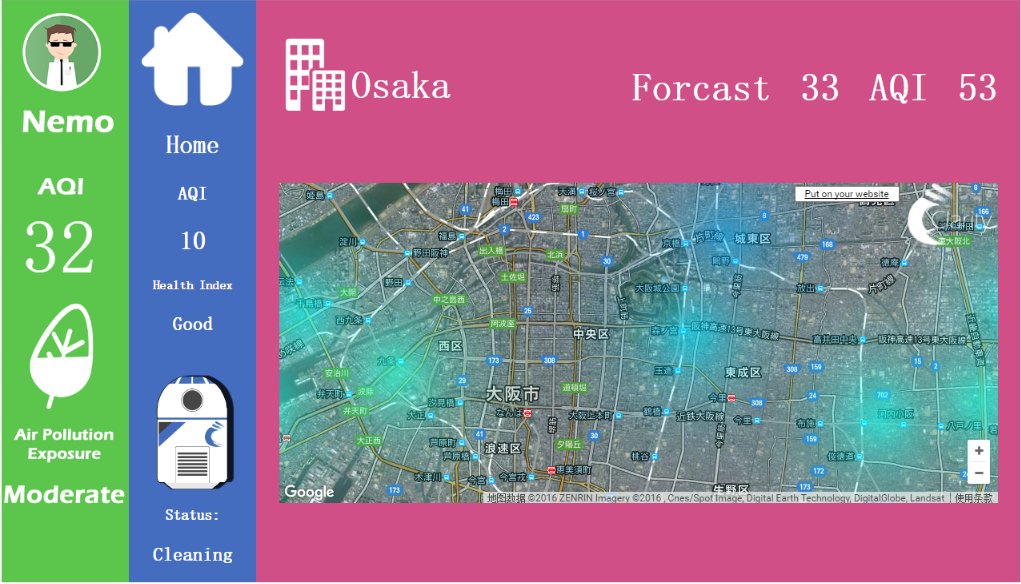
\includegraphics[width=\textwidth]{CityPanel.png}
 \bicaption[fig:CityPanel]{CityPanel组件}{CityPanel组件}{Fig}{CityPanel Component}
\end{figure}